\documentclass[12pt,a4paper,oneside]{memoir}
\usepackage[utf8]{inputenc}
\usepackage{background}
\usepackage{lipsum}% just to generate filler text
\usepackage{scrextend}
\usepackage{graphicx}

\usepackage[left=1.5cm,right=1.5cm,top=2cm,bottom=3cm]{geometry}

\usepackage{fancyhdr}
\pagestyle{fancy}
\usepackage{graphicx}
\usepackage{xcolor}
\usepackage{booktabs}
\usepackage[section]{placeins}
\usepackage{float}
\usepackage{mathptmx}
\usepackage{tocloft}
\usepackage{setspace}
\usepackage{pgfplots} %Histogram graphing
\usepackage{titlesec} %Title spacing
\usepackage{caption}
\usepackage{hyperref}
\usepackage{changepage}
\usepackage{color,soul}
\usepackage{xcolor}
\usepackage{gensymb}

\usepackage{lipsum}
\setlength\headheight{35pt} %% just to make warning go away. Adjust the value after looking into the warning.




\pgfplotsset{
  compat=newest,
  xlabel near ticks,
  ylabel near ticks
}


\SetBgContents{Prepared by Brady Planden, 2019}
\SetBgScale{1}
\SetBgAngle{0}
\SetBgOpacity{1}
\SetBgColor{black}
\SetBgPosition{current page.south west}
\SetBgHshift{4cm}
\SetBgVshift{1cm}

%\fancyhf{}
\lhead{
\includegraphics[width=1.25cm]{OBR_Logo.png}}
%\renewcommand{\headrulewidth}{0.4pt}


\mainmatter
\counterwithout{figure}{chapter}
\counterwithout{table}{chapter}


\begin{document}
\section*{Thermal Analysis of HV Cabling}
\begin{flushleft}
{\textbf{Notes\\}}
{This is a heat transfer analysis of $16 mm^2$, $20mm^2$, and $25mm^2$ standard Coroplast 1000V DC cable. This analysis uses the below equation to predict temperature gain found in "Fundamentals of Heat and Mass Transfer 7th ed.".\\}
\vspace{0.5cm}
\begin{centering}
{$ \frac{dT}{dt}=\frac{I^2R_e'-\pi Dh(T-T_\infty)-\pi D\epsilon\sigma(T^4-T_{surr}^4)}{\rho c(\pi D^2/4)}$\\}
\end{centering}
{Where:\\
I = Current\\
$R_e$ = Specific Electric Resistance\\
D = Conductive Core Diameter\\
h = Convection Coefficient\\
$\epsilon$ = Emissivity\\
$\sigma$ = Boltzmann Constant\\
$\rho$ = Conductor Density\\
T = Conductor Temperature\\
$T_{\infty}$ = Black Box Temperature\\
$T_{surr}$ = Ambient Surrounding Temperature\\
}
\vspace{0.5cm}
{The above equation is solved in Matlab and a current profile from a worst case Autocross run is applied. This profile assumes thermal constraints from the tractive system are not active (i.e. motor derating) and a step torque request during all straights in the 2015 Michigan Endurance course (reverse Autocross course). This profile also assumes a 600V pack.\\
\vspace{0.25cm}
The initial conductor temperature is assumed to be at ambient for this analysis, with the ambient temperature increases through the simulation from 303K to 318K.\\
\vspace{0.25cm}
The Coroplast 1000VDC cable has the following characteristics: }
\end{flushleft}

\begin{table}[H]
  \centering
  \captionsetup{aboveskip=0pt,font=it}
  \caption{Coroplast Characteristics}
  \resizebox{0.6\textwidth}{!}{   %resize table
    \begin{tabular}{cccc}
    \toprule
     \textbf{Cross Section [$mm^2$]} & \textbf{Diameter [mm]} & \textbf{Resistance [m\ohm/m]} & \textbf{Max Temperature [K]}\\
     16 & 5.8 & 1.16 & 453 \\
     20 & 6.9 & 0.96 & 453\\
     25 & 7.2 & 0.743 & 453\\
    \bottomrule
    \end{tabular}
    }
    \end{table}
    
\newpage
\begin{figure}[p]
\centerfloat
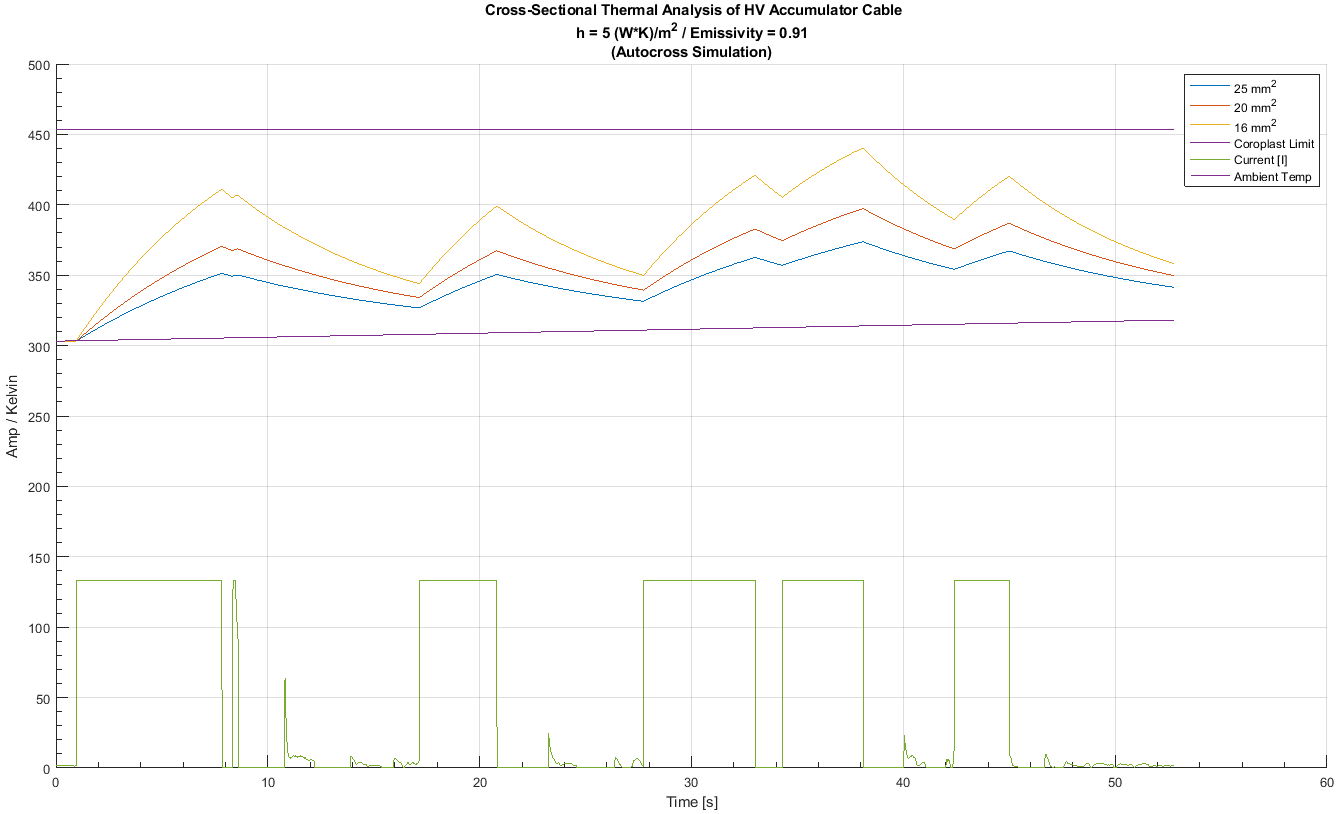
\includegraphics[width=1.0\textwidth]{Wire_Cross_Sectional_5h}
\captionsetup{aboveskip=0pt,font=it}
\caption{Autocross HV Cable Simulation with a Convection Coefficient of $5 \frac{W}{m^2}K$}
\label{Fig1}
\end{figure}

\newpage
\begin{figure}[p]
\vfill
\centerfloat
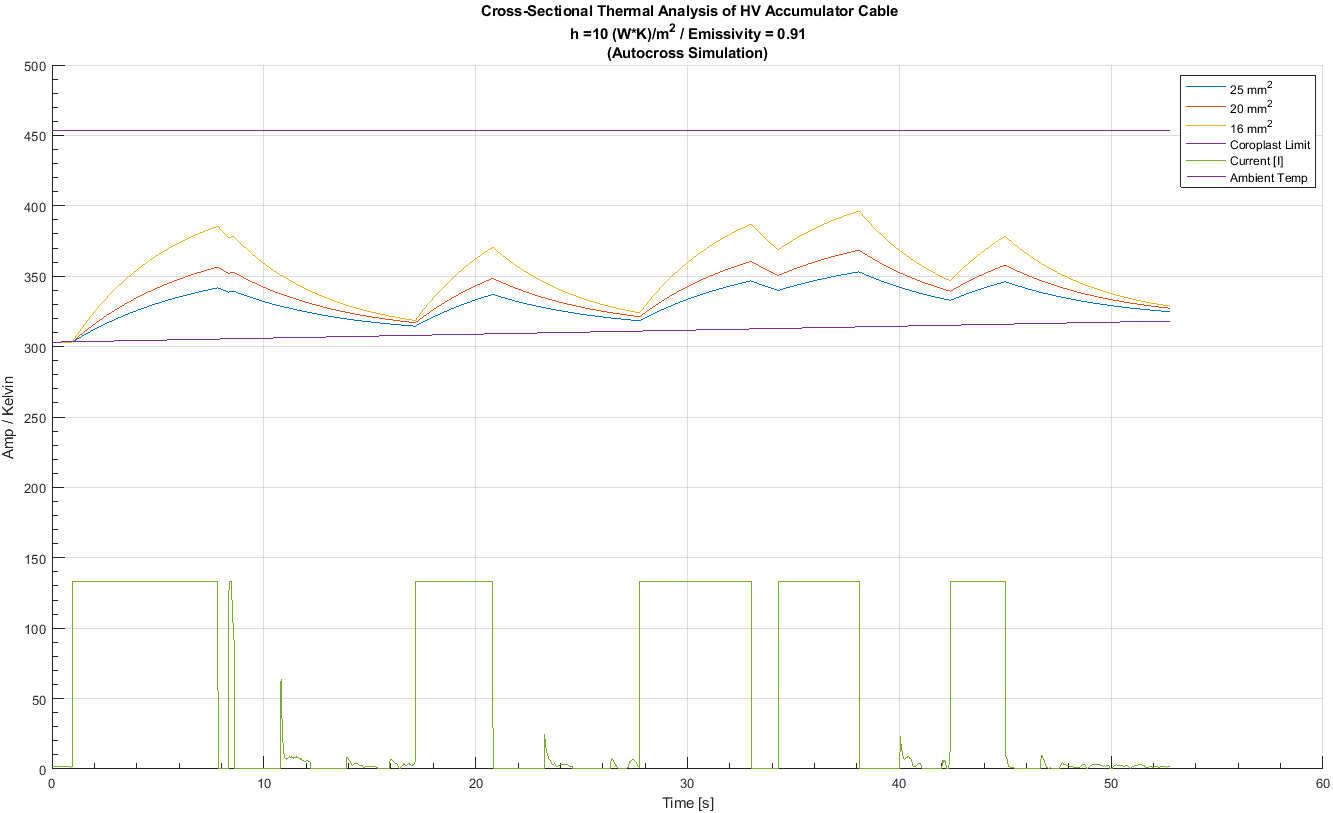
\includegraphics[width=1.0\textwidth]{Wire_Cross_Sectional_10h}
\captionsetup{aboveskip=0pt,font=it}
\caption{Autocross HV Cable Simulation with a Convection Coefficient of $10 \frac{W}{m^2}K$}
\label{Fig1}
\end{figure}



% \begin{figure}[!htbp]
% \centering
% \includegraphics[width=\textwidth]{445N_IA.jpg}
% \captionsetup{aboveskip=0pt,font=it}
% \caption{16" @ 445N Fz / Varying IA / 12 PSI}
% \label{Fig1}
% \end{figure}

% \begin{figure}[!htbp]
% \centering
% \includegraphics[width=\textwidth]{670N_IA.jpg}
% \captionsetup{aboveskip=0pt,font=it}
% \caption{16" @ 650N Fz / Varying IA / 12 PSI}
% \label{Fig1}
% \end{figure}

% \begin{figure}[!htbp]
% \centering
% \includegraphics[width=\textwidth]{1110N_IA.jpg}
% \captionsetup{aboveskip=0pt,font=it}
% \caption{16" @ 1050N Fz / Varying IA / 12 PSI}
% \label{Fig1}
% \end{figure}

% \begin{figure}[!htbp]
% \centering
% \includegraphics[width=\textwidth]{1110N_IA_3D.jpg}
% \captionsetup{aboveskip=0pt,font=it}
% \caption{16" @ 1050N Fz / Varying IA / 12 PSI - Showing Transitional IA}
% \label{Fig1}
% \end{figure}


\end{document}
